\label{chapter:starcraftmultiagentchallenge}
% Please refereer ook naar je main artikel, a.k.a. het artikel waarin je dit allemaal hebt gevonden
\subsection{About} 
Real world tasks often consist of multiple agents with each their own observations and limited communications to other agents. In recent years the amount of research
done in this field has increased exceptionally, however it is difficult to benchmark the progress because  most
papers use their own one-off problems. Standardized environments for single-agent reinforcement learning have enabled great progress. Some testbeds have emerged for multi-agent problems such as Poker\citep{heinrich2016deep}, Pong\citep{tampuu2017multiagent} or Keepaway Soccer\citep{stone2005keepaway}. Nonetheless, there is still a clear lack of standardized testbeds for research and evaluation. This led to Samvelyan et al.\citep{samvelyan2019starcraft} proposing the StarCraft Multi-Agent Challenge (SMAC). The team behind SMAC also released an open-source deep multi-agent reinforcement learning learning framework including state-of-the-art algorithms.

A great deal of environments have been created to develop and test multi-agent reinforcement learning(MARL) agents. However, not many of these provide elements of strong partial observability, challenging dynamics and high-dimensional observation spaces. SMAC is based on the popular real-time strategy (RTS) game StarCraft II and aims to prove all these elements. SMAC consists of micromanagement tasks where a team of agents need to work together to achieve a common goal. The micromanagement tasks require that each unit be controlled by its own agent and they should cooperate to complete the task. Because the learning proceeds in a simulation the algorithm has access to the full global state, this makes it possible for the training to be conducted in a centralized fashion while the execution still conditions on decentralized local observations. A number of recent state-of-the-art algorithms use this paradigm of \textit{centralised training with decentralised execution} to speed up the learning of decentralized policies. Roughly speaking, a policy defines what actions to take when the agent is in an arbitrary state of the environment. Among these are COMA\citep{foerster2018counterfactual} an actor-critic algorithm and QMIX\citep{rashid2018qmix} which belongs to the Q-learning family.

\subsection{Applied Methods and Techniques}

As described in previous section, SMAC is a testing environment. In this section, the different techniques that have been tested in the environment are summarized and explained.

\subsubsection{Independent Q learning\citep{tan1993multi}}

Independent Q learning (IQL) is based on the idea that humans do not need to learn everything from scratch but can share information. If a task is too big for a single agent to solve they will cooperate to achieve their common goal. To create IQL each agent uses the one step Q learning algorithm\citep{watkins1992q} and extends it to multiple independent agents. Q learning is a reinforcement learning algorithm that uses a table where the columns are the possible actions and the rows are the states. Each cell will contains the value of the maximum expected future reward when picking that action for a specific state. Q learning is an iterative process where the agent picks an action based on the table, performs the chosen action, measures the reward and updates the table with the new value. The IQL paper identifies three ways of getting these reinforcement learning agents to cooperate:
\begin{itemize}
   \item  Agents can communicate instantaneous information such as observations, actions or rewards.
   \item  Agents can communicate episodes that are sequences of triples (observation, action, reward) experienced by agents.
   \item  Agents can communicate learned decision policies.
\end{itemize}

To test this, a 10 by 10 grid world was created. In this world a hunter needs to locate and capture a prey. The prey moves randomly and the hunter has a limited view of the world. The initial test showed that a hunter that was learning outperformed a hunter that moved randomly. Adding another agent called Scout, which can not capture the prey but can communicate its own local observations with the hunter improved the performance once again. This proved the benefit of additional local observations and this idea could be extended to two hunters. A test with two hunters showed that observations from another agents should be used carefully and that insufficient information can hinder the learning. Two mutual-scouting hunters outperform two independent hunters in execution. But a scouting hunter with a field of view of 2 cells can not keep up the the prey long enough for the other hunter to learn to catch up, this causes the mutual-scouting hunters to perform worse in training.

Instead of cooperation through exchanging observations instantaneously agents could share a decision policy. When agents use the same decision policy it greatly improves the time it takes to train. Even though the independent agents eventually will reach the same level as performance. The decision policy is kept by a single agent, this particular agent receives the observations of all other agents and sends them the action they should execute. After the agents execute the action they will send the decision policy keeping agent the reward for that action.

Another approach is having agents exchange episodes of what they have experienced. When a hunter captures a prey it transfer everything it has learned so far to the other hunter. The other hunter replay this to update their own decision policy. This results in the two hunters doubling their learning experience. When the episodes received come from a expert hunter it improved the learning rate additionally.

\subsubsection{Decentralized partially observable markov decision process (Dec-POMDPs)\citep{oliehoek2016concise}}

Both COMA and QMIX consider Dec-POMDPs which can be used to describe fully cooperative multi-agent tasks. A Dec-POMDP consists of a tuple $G = \langle S,U,P,r,Z,O,n, \gamma  \rangle$. $s \in S$ describes the true state of the environment. At each time step, each agent simultaneously chooses an action $u^{a} \in U$, forming a joint action $u \in U \equiv U^{n}$ which causes a transition in the environment according  to  the  state  transition  function
$P(s'|s, \textbf{u}) : S \times \textbf{U} \times S \rightarrow [0,1]$. The agents all share the same reward function r(s, \textbf{u}) :  $S \times \textbf{U} \rightarrow {\rm I\!R}$ and $\gamma \in [0,1]$ is a discount factor.
\newline
\newline
We  consider  a  partially  observable  setting,  in  which agents  draw  observations $z \in Z$ according  to  the  observation function $O(s,a) : S \times \textbf{A} \rightarrow Z$. Each agent has an action-observation history $\tau^{a} \in T \equiv (Z \times U)*$, on which it conditions a stochastic policy $\pi^{a}(u^{a}|\tau^{a}) : T \times U \rightarrow [0,1]$. The joint policy $\pi$ has a joint action-value function: $Q^{\pi}\left(s_{t}, \mathbf{u}_{t}\right) = \mathbf{E}_{s_{t+1 : \infty}, \mathbf{u}_{t+1 : \infty}}\left[R_{t} | s_{t}, \mathbf{u}_{t}\right]$, with $R_{t}=\sum_{i=0}^{\infty} \gamma^{i} r_{t+i}$ being the discounted return.

\subsubsection{Counterfactual Multi-Agent Policy Gradients}

Like mentioned before, COMA is an algorithm that trains centralized but executes decentralized. COMA takes the actor-critic\citep{NIPS1999_1786} approach. The actor-critic method uses two neural networks, a critic that approximates how good the taken action is and an actor who controls the behaviour of our agent. The actor is trained using a gradient that's estimated by the critic. To have this apply to multiple agents each agent has to learn independently from its own critic and action. This is the same idea as independent Q-learning, but using the actor-critic model instead of Q-learning. COMA is based on three main ideas. First, COMA uses a centralized critic. The critic is only used in training. During the execution, the agents make their own choices based on their own local observations. The equation to calculate the gradient is:
\begin{equation} \label{eq:coma}
g=\nabla_{\theta^{\pi}} \log \pi(u | \tau_{t}^{a})\left(r+\gamma V\left(s_{t+1}\right)-V\left(s_{t}\right)\right)
\end{equation}

The estimate of the gradient is specific to each agent. The left side of the equation(\ref{eq:coma}) is specific to each agents decentralized policy and its action based on local observations. The right side of the equation(\ref{eq:coma}) is computed using a centralized critic, that depends on the global state that is only visible to the critic during training. 

Second, COMA solves the multi-agent credit assignment, by using an counterfactual baseline which is inspired by difference rewards\citep{wolpert2002optimal} \citep{tumer2007distributed}. The multi-agent credit assignment is figuring out how much a specific agent contributed towards the teams goal. Difference rewards are used to calculate the contribution of a single agent towards the teams goal. This is done by comparing the received reward with the reward that would have been received if the agent executed an default action. This reward function has limitations, to estimate the difference rewards it needs to run two simulation, one with the agent contributing and one where the agent executes the default action. Another limitation is deciding on a default action that best approximates its absence in the system. The counterfactual baseline addresses both these limitations.

\begin{equation} \label{eq:coma2}
g_{a}(\tau)=\sum_{t=0}^{T} \nabla_{\theta} \log \pi_{\theta}\left(u_{t}^{a} | \tau_{t}^{a}\right) A^{a}\left(s_{t}, \mathbf{u}_{t}\right)
\end{equation}
\begin{equation} \label{eq:comaA}
A^{a}(s, \mathbf{u})=Q(s, \mathbf{u})-\sum_{u^{\prime a}} \pi^{a}\left(u^{\prime a} | \tau^{a}\right) Q\left(s,\left(\mathbf{u}^{-a}, u^{\prime a}\right)\right)
\end{equation}

The computation that is done by the critic is replaced with an activation function(\ref{eq:comaA}) which is specific for every agent. The activation function uses the Q-value that's been estimated by the gradient and a counter factual Q-value that calculated by doing the following: for every action the agent could have taken in that state, what would the Q-value have been if the agent had taken that action instead. Actions are marginalized by considering all actions the agents could have taken weighted by the probability it would have taken them based on its current policy. With the updated equation (\ref{eq:coma2}) the limitations are no longer relevant since the default action has been removed. Since all the information needed is already present within the critic, no extra simulations are needed. 

The calculation of the counter factual needs to happen in an efficient way. Using a neural network, which would use as input the state and joint action and produce as output the team reward for the specific action taken by the agent. A neural network like this needs to do a forward pass, calculating a Q value for each action the agent could have taken, which is costly. Another approach is the one used by Deep Q-Networks where the input is just the state and there's an output for every action. With this approach the number of outputs would be massive. What COMA does instead is take the representation of the actions taken only by the other agents and it produces the value of the joint action when that joint action is completed by each of the different actions available to the agent whose contribution is calculated. So this means that in one forward pass we calculate the Q-value for each action in the summation.

\subsubsection{QMIX}

%maybe weglaten of iets dieper of ingaan
Independent Q learning cannot clearly represent interactions between the agents and COMA requires on-policy, which means the Q-value gets updated using the next state and the current action based on it's policy. This may cause COMA to be sample-inefficient, needing a lot of samples to learn, and training the centralized critic can become impractical with the growing amount of agents.
%maybe weglaten

QMIX is very much like value decomposition networks\citep{sunehag2017value}, VDN learns a centralized, but factored expected team reward: $Q\textsubscript{tot}$. Each agent has an individual value function $Q\textsubscript{a}$ which conditions on that agents individual actions and observations. A decentralized policy is created by each agent greedily selecting actions with respect to its $Q\textsubscript{a}$. $Q\textsubscript{tot}$ is a summation of these individual $Q\textsubscript{a}$  values. The key method of QMIX is that the full factorization that VDN does is not needed to create decentralized policies. QMIX also has a much richer class of action-value functions unlike the functions from VDN which are severely limited in complexity.

QMIX is created by having agent networks represent each $Q\textsubscript{a}$ and a mixing network, which is a feed-forward neural network that takes the agents output and mixes them monotonically to create $Q\textsubscript{tot}$. Unlike a VDN which uses a simple sum to create $Q\textsubscript{tot}$, QMIX does this in a complex non-linear way so that there is consistency between the centralized an decentralized policies. 

Each agent network is represented as deep recurrent Q-networks that receive current local observations $o^{a}_{t}$ and the last action $u^{a}+{t-1}$ as input at each time-step.

The weights of the mixing network are produced by separate hypernetworks. Hypernetworks are networks that are used to generate the weights for another network. The weights of one layer of the mixing network are generated by using the state s as input for the hypernetwork. The hypernetworks consists of a single linear layer followed by an absolute activation function to ensure non-negative weights. The output is a vector that is reshaped into a matrix of appropriate size.

The biases that are produced in the same manner can be negative values. The final bias is produced by a 2 layer hypernetwork with a ReLU non-linearity.

The feed-forward mixing network have been replaced with recurrent neural network (RNN) mixing networks when testing the algorithm in the SMAC environment. The RNN improved the learning rate greatly while the final performance was relatively the same.

In figure \ref{fig:qmix} the network structure that was presented in the QMIX paper is showed.

\begin{figure}
  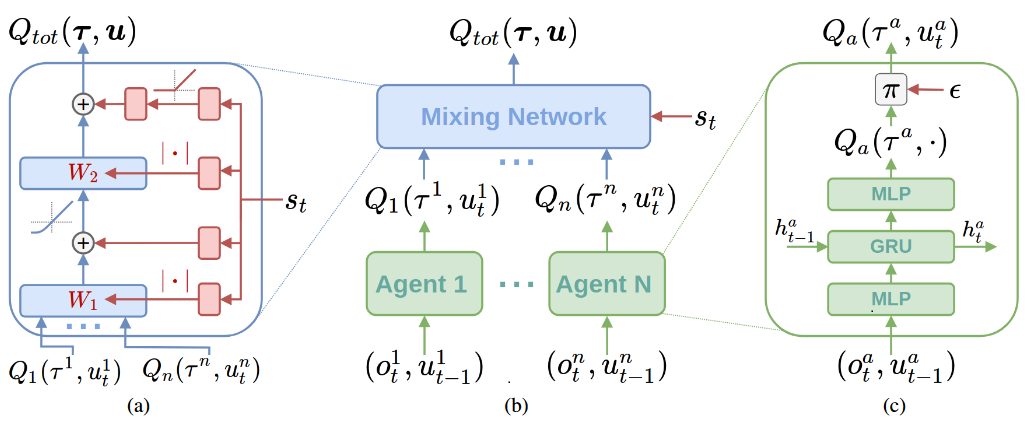
\includegraphics[width=\linewidth]{images/qmix.png}
  \caption{As presented in the QMIX paper: (a) Mixing network structure. In red are the hypernetworks that produce the weights and biases for mixing network layers showning blue. (b) The overall QMIX architecture. (c) Agent network structure. Best viewed in color}
  \label{fig:qmix}
\end{figure}

\subsection{Contributions to Reinforcement Learning}

Independent Q learning was one of the earliest attempts at multi-agent reinforcement learning and it's still the most commonly applied method for multi-agent learning. Two papers using a combination of IQL and Deep Q learning show strong results\citep{tampuu2017multiagent}\citep{leibo2017multi}. In IQL each agent has its own action-value function Q, however this approach does not clearly show the interactions between the agents. Multi-agent credit assignment is an interesting issue when it comes to decentralized cooperating agents. The approach taken by COMA is to take the existing reward function and remove the limitations while still being efficient.
QMIX takes another approach, $Q\textsubscript{tot}$ is the sum of all individual Q functions, one for each agent. But instead of using a simple sum, QMIX uses a monotic function.

\subsection{Future plans}
The next step for QMIX and COMA is to conduct additional tests with a larger number of agents. In COMAs case, centralized critics are harder to train and exploration becomes challenging. QMIX has plans to add more coordinated exploration schemes for settings with a larger number of learning agents. The SMAC environment is also planning on adding new challenging scenarios which require a high level of coordination between agents.